\chapter{Networking Introduction, Characteristics, and Types}

\section{Introduction to Networking}

A network is a collection of devices connected together with the ability to communicate with each other.

The benefits of a network is perhaps too obvious at the time of writing -- almost every element of life is supported by some form of a network. But still:

\begin{enumerate}
    \item Connectivity \& communication
    \item Sharing
    \item Internet access
    \item Data security
    \item Performance enhancing
    \item Entertainment
\end{enumerate}

There are also disadvantages, also quite obvious:

\begin{enumerate}
    \item Management/software costs
    \item Undesirable sharing
    \item Illegal activity
    \item Data security concerns
\end{enumerate}

\section{Fundamental Network Characteristics}

\textit{Networking Models} help us organize and manage what devices in a network do and how they interact. 

\begin{figure}[H]
    \centering
    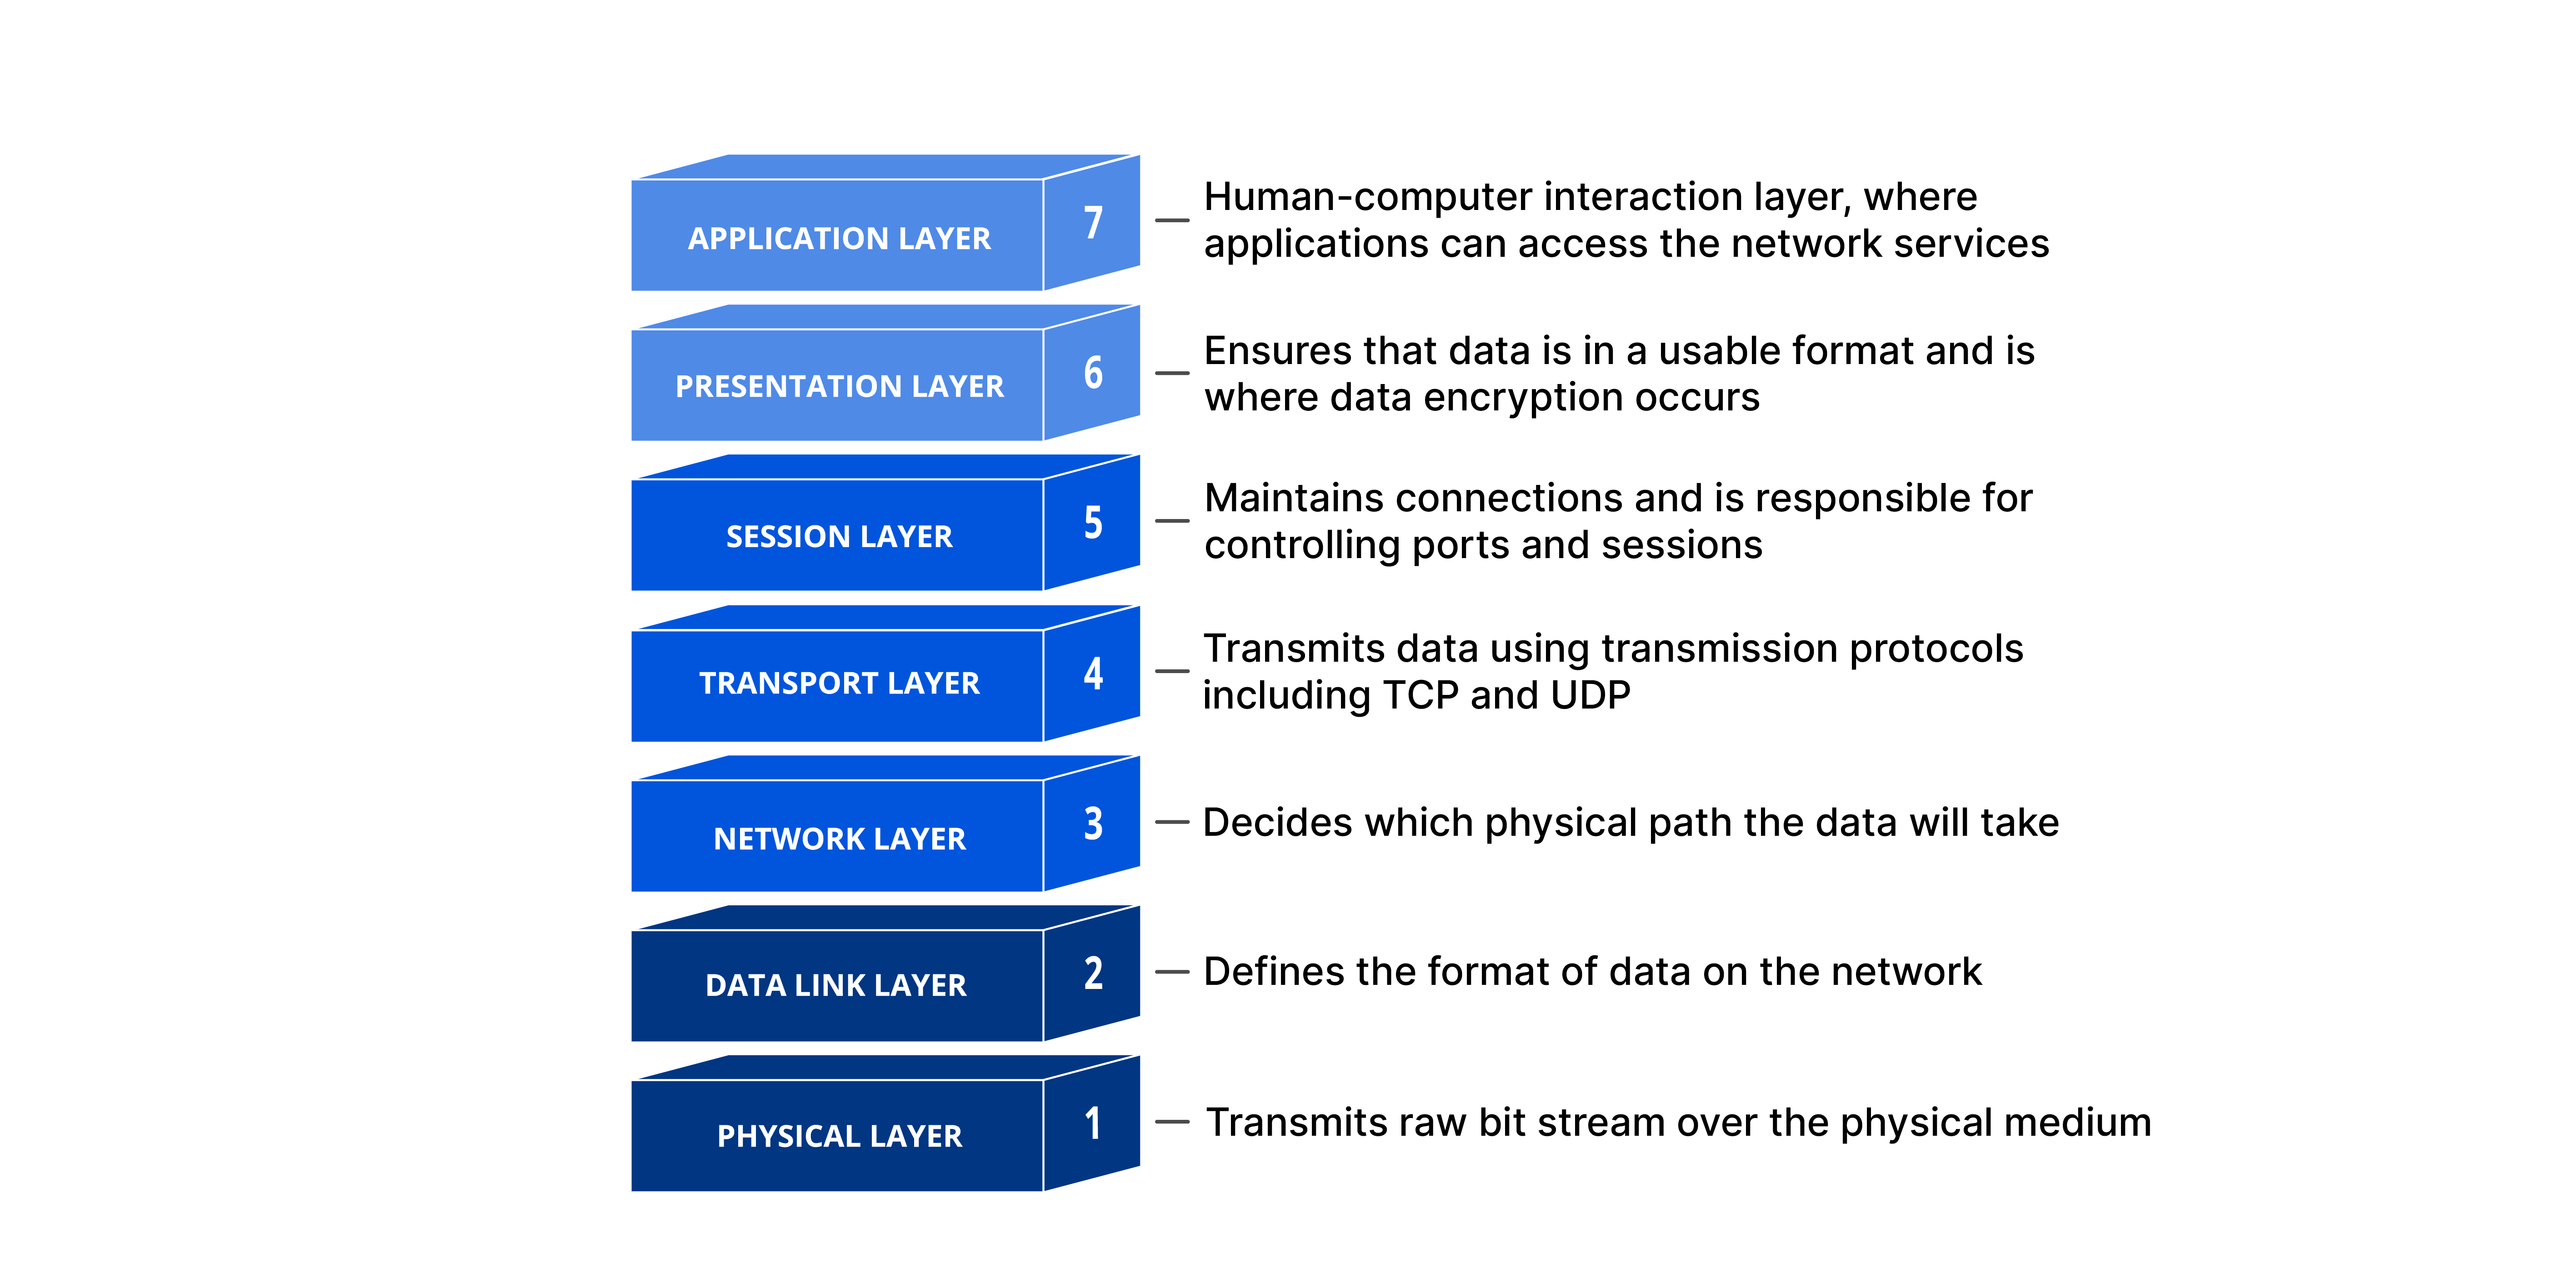
\includegraphics[width=\linewidth]{assets/osi-model.png}
    \caption{OSI Model\\
    \small \textit{Cloudflare}}
    \label{fig:label}
\end{figure}

The most common model is the \textit{Open Systems Interconnection} (OSI) reference model. These include the multiple layers at which networking can happen. From the top layer which concerns applications to the bottom layer where the physical transfer of bits are concerned.

\bigskip

\textit{Protocol} is a vague term that can mean a lot of things, from high-level protocols to low-level protocols. But, in essence, protocols are agreements that allow devices to communicate effectively. Agreeing on the same protocol is thus important.

\bigskip

There are two methods in which information gets passed along a network: \textit{circuit switching} and \textit{packet switching}.

\textit{Circuit switching} focuses on establishing a path between two devices and maintaining that connection for as long as they need. An analogous situation is phone lines, where once two devices establish a call, they should be on the line for as long as they want, and no other devices should be able to ``intervene'' with their connection.

\textit{Packet switching} focuses on sending information over a shared medium, where there is no definite path. This method is similar to the mail system, where all mail are sent through a common medium. Individual packets might take different paths to the destination, and as a disadvantages packets might get lost along the way (namely packet loss).

There isn't really preference in one over the other. But packet switching is the predominant method today (i.e. LAN).

\bigskip

Another difference is whether a connection is used: \textit{connection-oriented} and \textit{connectionless} protocols.

\textit{Connection-oriented} 